\chapter{Estrutura do documento}
A estrutura se refere à divisão de um documento em partes, capítulos, seções e níveis adicionais de estrutura.
\begin{figure}[h]
    \centering
    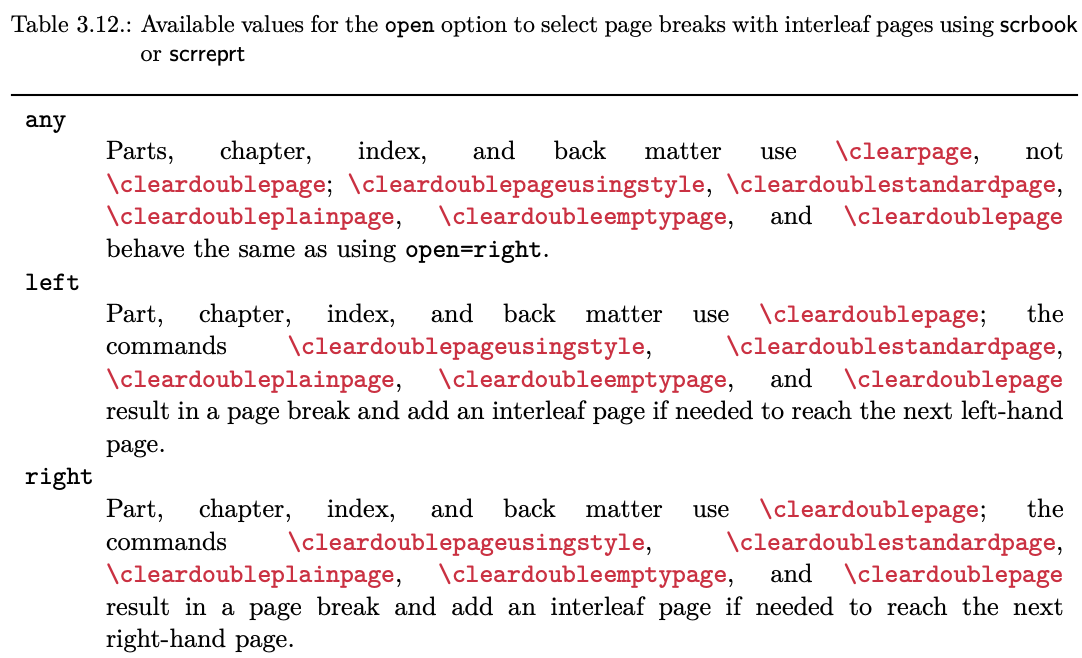
\includegraphics[width=0.80\linewidth]{imagem17.png}
    %\caption{Enter Caption}
    \label{fig:3_12}
\end{figure}

\minisec{open=method}
As classes \KOMAScript\ \texttt{scrbook} e \texttt{scrreprt} oferecem a você a opção de onde começar um novo capítulo com impressão frente e verso. Por padrão, \texttt{scrreprt} inicia um novo capítulo na próxima página. Isso é equivalente ao método any. No entanto, \texttt{scrbook} inicia novos capítulos na próxima página à direita. Isso é equivalente ao método right e geralmente é usado em livros. Mas às vezes os capítulos devem começar na página esquerda de uma página dupla. Você pode fazer isso com o método left. Você pode encontrar um resumo dos valores disponíveis na tabela 3.12. A tabela também descreve os efeitos de \char`\\\texttt{clear\-dou\-ble\-pa\-ge}, \char`\\\texttt{clear\-dou\-ble\-pa\-ge\-u\-sing\-sty\-le}, \char`\\\texttt{clear\-dou\-ble\-stan\-dard\-pa\-ge}, \char`\\\texttt{clear\-dou\-ble\-plain\-pa\-ge} e \char`\\\texttt{clear\-dou\-ble\-empty\-pa\-ge} (consulte a seção 3.13, página 87).

Como o \LaTeX\ não diferencia entre páginas esquerdas e direitas na impressão de um lado, a opção não tem efeito nesse caso.

Na classe \texttt{scrartcl}, a seção é o primeiro elemento estrutural abaixo da peça. Por esse motivo, \texttt{scrartcl} não suporta essa opção.

\begin{figure}
    \centering
    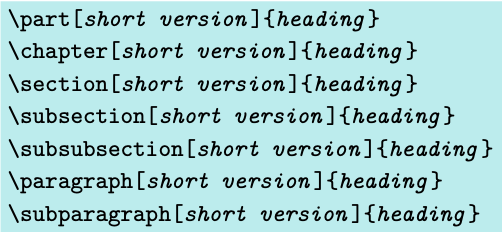
\includegraphics[width=0.65\linewidth]{imagem18.png}
    \label{fig:img18}
\end{figure}

Os comandos de seccionamento padrão no \KOMAScript\ funcionam da mesma forma que aqueles nas classes padrão. Assim, você pode especificar um texto alternativo para o índice e títulos como um argumento opcional para os comandos de seccionamento.

No entanto, com a opção \texttt{headings=optiontohead}, o \KOMAScript\ usa apenas a versão curta do argumento opcional no título, não no índice. Claro, esse texto só aparecerá se você usar um estilo de página que coloque o nível de seccionamento correspondente no título. Veja a seção 3.12 e o capítulo 5. Com a opção \texttt{headings=optiontotoc}, o \KOMAScript\ usa a versão curta (\textit{short version}) do argumento opcional exclusivamente para o índice e não para o título. No entanto, a entrada será mostrada apenas se o \texttt{tocdepth counter} for grande o suficiente (veja a seção 3.9, página 76). Com a opção \texttt{headings=optiontoheadandtoc}, o \KOMAScript\ usa a versão curta do argumento opcional tanto no índice quanto no título. Todas essas três opções ativam a interpretação estendida da versão curta do argumento opcional, que não está ativa por padrão.

A interpretação estendida do argumento opcional verifica se há um sinal de igual na versão curta. Se houver, o argumento opcional será interpretado como uma lista de opções. Quatro opções
\begin{itemize}
    \item \texttt{head=running head},
    \item \texttt{tocentry=table of contents entry},
    \item \texttt{reference=reference title} e 
    \item \texttt{nonumber=simple switch}
\end{itemize}

são suportadas com este formato. Para usar vírgulas ou sinais de igual dentro dos valores dessas opções, você deve colocá-los entre chaves.

Observe que este mecanismo só funciona enquanto o \KOMAScript\ controlar os comandos de seccionamento. Se você usar um pacote que redefine os comandos de seccionamento do \KOMAScript\ ou do kernel interno do \LaTeX, o \KOMAScript\ não poderá mais fornecer este mecanismo estendido. Isso também se aplica a uma extensão do \KOMAScript\ que está sempre ativa: comandos de seccionamento sem texto de título não criam entradas no índice. Se você realmente quiser uma entrada com texto de título vazio, você pode usar uma entrada invisível como \mbox{}.

\textbf{Exemplo}: Suponha que você tenha um documento com títulos de capítulo muito longos. Esses títulos devem aparecer no índice, mas você quer limitar o título corrente a títulos curtos de uma única linha. Você pode fazer isso com o argumento opcional de \char`\\\texttt{chap\-ter}.

\begin{figure}[h]
    \centering
    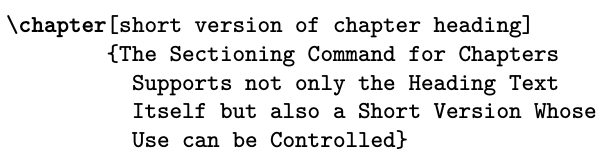
\includegraphics[width=0.60\linewidth]{imagem14.png}
    \label{fig:img14}
\end{figure}

Um pouco mais tarde, você percebe que as quebras de linha para esse longo título são muito inapropriadas. Portanto, você quer escolher as quebras você mesmo. No entanto, você ainda quer quebra de linha automática no índice. Com
\begin{figure}[h]
    \centering
    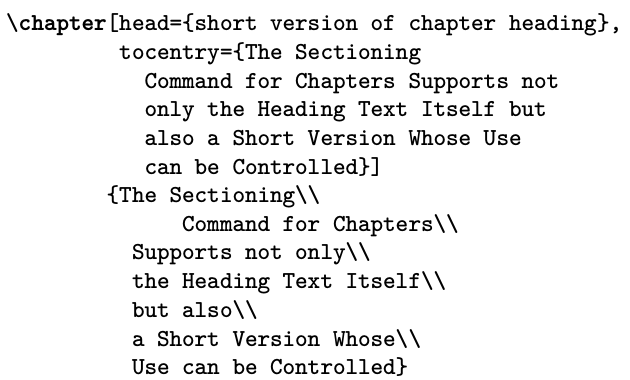
\includegraphics[width=0.60\linewidth]{imagem19.png}
    %\caption{Enter Caption}
    \label{fig:img19}
\end{figure}

você cria entradas separadas para o índice, título corrente e o próprio título do capítulo. Os argumentos das opções head e tocentry foram colocados entre chaves para que seus conteúdos possam ser arbitrários.

É possível usar diferentes tipos de fonte para diferentes níveis de seccionamento no KOMA-Script. Não especialistas em tipografia devem evitar fazer isso por excelentes razões tipográficas.

Uma regra da tipografia afirma que você deve misturar o mínimo de fontes possível. Usar \textit{sans serif} para títulos já parece violar essa regra. No entanto, você deve perceber que letras grandes, em negrito e \textit{serif} são muito pesadas para títulos. A rigor, você deve usar uma fonte normal em vez de uma fonte em negrito ou seminegrito. No entanto, em níveis mais profundos do seccionamento, uma fonte normal pode então parecer muito clara. Por outro lado, fontes \textit{sans serif} têm uma aparência muito agradável em títulos, e quase exclusivamente em títulos. Há, portanto, uma boa razão pela qual \textit{sans serif} é o padrão no \KOMAScript.

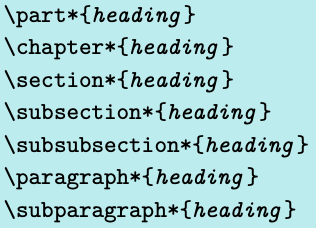
\includegraphics[width=0.40\linewidth]{imagem20.png}

As variantes com estrela de todos os comandos de seccionamento produzem títulos não numerados que não aparecem no índice ou no cabeçalho contínuo. A ausência de um cabeçalho contínuo geralmente tem um efeito colateral indesejado. Se, por exemplo, um conjunto de capítulos usando \verb|\chapter*| abrange várias páginas, então o cabeçalho contínuo do capítulo anterior reaparece repentinamente. O \KOMAScript\ oferece uma solução para esse problema, descrita abaixo. \verb|\chapter*| só existe nas classes book e report, ou seja, book, scrbook, report e scrreport, não nas classes article e scrartcl.

Observe que \verb|\part| e \verb|\chapter| alteram o estilo de página para uma página. Enquanto as classes padrão usam o estilo de página simples, o \KOMAScript\ aplica o estilo definido nas macros \char`\\\texttt{part\-pa\-ge\-sty\-le} e \char`\\\texttt{chap\-ter\-pa\-ge\-sty\-le} (veja a seção 3.12, página 83).

As possibilidades de troca de fontes mudam. Os elementos usam os mesmos nomes, pois não indicam variantes, mas níveis de estruturação.

\section{Minisec}
\begin{verbatim}
   \minisec{heading} 
\end{verbatim}

Às vezes, você quer um título que seja destacado, mas também intimamente vinculado ao texto seguinte. Tal título não deve ser separado por um grande salto vertical.

O comando \verb|\minisec| é projetado para esta situação. Este título não é associado a nenhum nível de seccionamento. Tal minisseção não produz uma entrada no índice, nem recebe nenhuma numeração.

Você pode alterar a fonte do comando \verb|\minisec| usando o elemento \texttt{disposition} e \texttt{minisec} (veja a tabela 3.2, página 59). O padrão do elemento \texttt{minisec} é vazio, então por padrão somente o elemento \texttt{disposition} é usado.

\textbf{Exemplo}: Você desenvolveu um kit para construir uma ratoeira e quer a documentação separada em uma lista de itens necessários e uma descrição de montagem. Você pode escrever o seguinte:

\begin{figure}
    \centering
    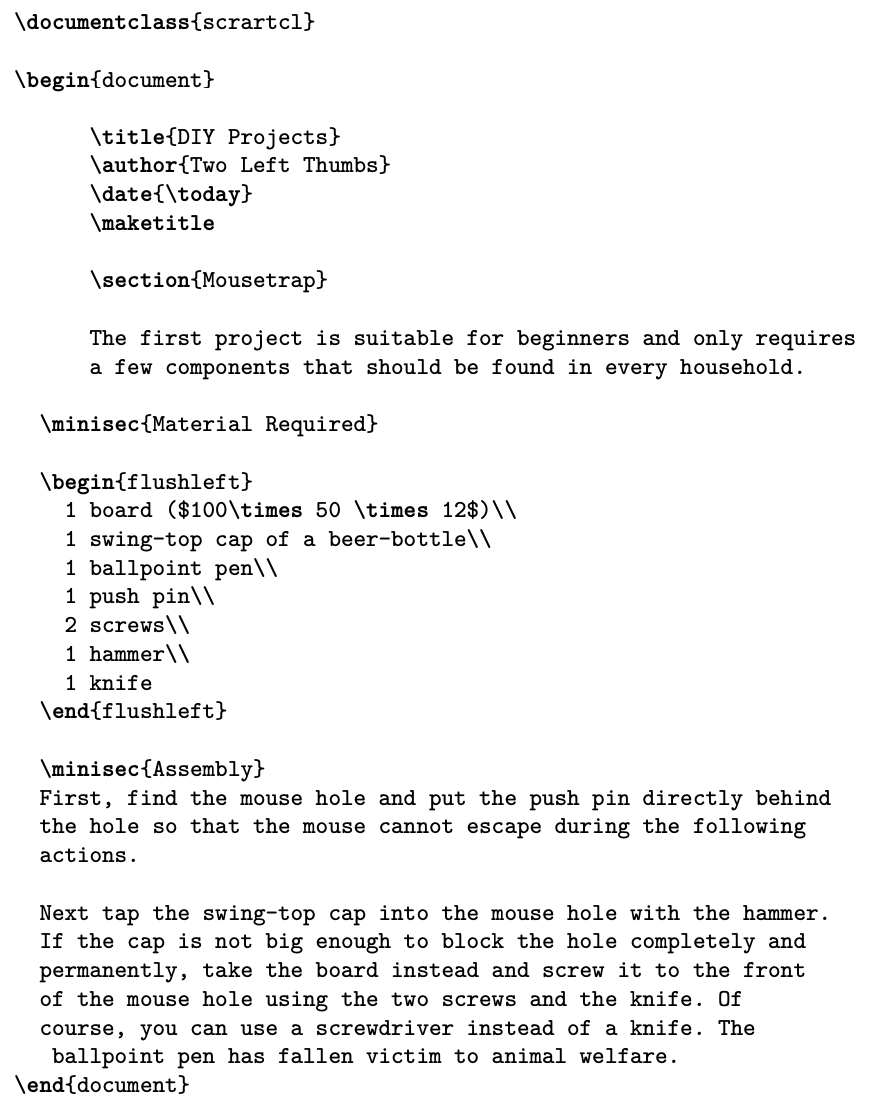
\includegraphics[width=0.8\linewidth]{imagem21.png}
    %\caption{Enter Caption}
    \label{fig:img21}
\end{figure}

\begin{figure}
    \centering
    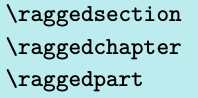
\includegraphics[width=0.4\linewidth]{imagens/imagem22.png}
\end{figure}

\newpage

Nas classes padrão, os títulos são definidos como texto justificado. Isso significa que palavras hifenizadas podem ocorrer e títulos de várias linhas são esticados até a largura do texto. Essa abordagem é bastante incomum em tipografia. O \KOMAScript\ portanto, define os títulos alinhados à esquerda com recuo deslocado usando \char`\\\texttt{ragged\-sec\-tion} com o padrão:
\begin{verbatim}
    \newcommand*{\raggedsection}{\raggedright}
\end{verbatim}

Você pode redefinir este comando com \char`\\\texttt{renewcommand}.

\textbf{Exemplo}: você prefere títulos justificados, então você escreve no preâmbulo do seu documento:
\begin{verbatim}
    \renewcommand*{\raggedsection}{}
\end{verbatim}
ou mais compactamente:
\begin{verbatim}
    \let\raggedsection\relax
\end{verbatim}

Você obterá uma formatação de título muito próxima daquela das classes padrão. Ela ficará ainda mais próxima quando você combinar essa alteração com a alteração no elemento de disposição mencionado acima.

Porque alguns usuários querem um alinhamento diferente para o nível \verb|\chapter| do que para os outros níveis de seção, você pode alterar a justificação \verb|\chapter| separadamente redefinindo \char`\\\texttt{rag\-ged\-chap\-ter}. Por padrão, no entanto, este comando simplesmente usa \char`\\\texttt{rag\-ged\-sec\-tion}, então alterar \char`\\\texttt{rag\-ged\-sec\-tion} afeta indiretamente \char`\\\texttt{rag\-ged\-chap\-ter}.

Por padrão, os títulos de parte (\verb|\part|) são definidos horizontalmente centralizados em vez de irregulares à direita. Esta formatação é realizada pela declaração \verb|\raggedpart|, que tem a definição padrão
\begin{verbatim}
    \let\raggedpart\centering
\end{verbatim}


Você também pode redefinir este comando usando \verb|\renewcommand|.

\textbf{Exemplo}: Você quer que os títulos para \verb|\part| sejam formatados da mesma forma que qualquer outro comando de seção. Para fazer isso, coloque
\begin{verbatim}
    \renewcommand*{\raggedpart}{\raggedsection}
\end{verbatim}

no preâmbulo do seu documento. Neste caso, e diferente do exemplo acima, nós não usamos \verb|\let| porque \verb|\let| definiria \char`\\\texttt{rag\-ged\-part} para o valor subjacente de \char`\\\texttt{rag\-ged\-sec\-tion}. Alterações subsequentes em \char`\\\texttt{rag\-ged\-sec\-tion} não mudariam o comportamento de \char`\\\texttt{rag\-ged\-part}. Ao redefinir com \char`\\\texttt{re\-new\-com\-mand}, \char`\\\texttt{rag\-ged\-part} usará o significado atual de \verb|\raggedsection| no momento em que for usado, em vez de quando foi redefinido.

\begin{figure}
    \centering
    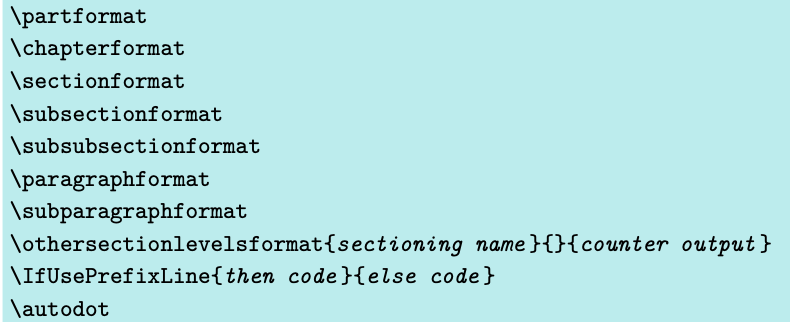
\includegraphics[width=0.8\linewidth]{imagem23.png}
\end{figure}

O \KOMAScript\ adiciona outra camada lógica acima do nome \char`\\\texttt{the\-sec\-tio\-ning} para formatar os números de seccionamento. Os contadores para cada título não são meramente emitidos. Eles são formatados usando os comandos \char`\\\texttt{part\-for\-mat}, \char`\\\texttt{chap\-ter\-for\-mat}, até \char`\\\texttt{sub\-pa\-ra\-graph\-for\-mat}. Claro, o comando \char`\\\texttt{chap\-ter\-for\-mat}, como \verb|\thechapter|, não existe na classe scrartcl, mas apenas nas classes scrbook e scrreprt.

Como já explicado para a opção numbers no início desta seção (veja a página 99), o tratamento de pontos do \KOMAScript\ em números de seção implementa as regras fornecidas em [DUD96], que são padrão na tipografia de língua alemã, no comando \verb|\autodot|. Em todos os níveis exceto para \verb|\part|, um ponto é seguido por um \verb|\enskip| adicional. Isso corresponde a um salto horizontal de 0.5em.
